\documentclass[14pt]{beamer}

\mode<presentation>{ \usetheme{Madrid}

% To remove the navigation symbols from the bottom of all slides uncomment next line
\setbeamertemplate{navigation symbols}{}
\date{}
\title{}
\author{}

%to get rid of footer entirely uncomment next line
\setbeamertemplate{footline}{}
}

\usepackage{geometry}
\usepackage{multirow}
\usepackage{adjustbox}
\usepackage{multicol}
\setlength{\columnsep}{0.1cm}

\usepackage{tikz}
\usetikzlibrary{shapes, backgrounds}

\usepackage{bbding}
\usepackage{rotating}
\usepackage{xcolor}

%\usepackage{tkz-berge} %cool grid
\usepackage{pgfplots} %pics

\usepackage{graphicx} % Allows including images
\usepackage{
	booktabs
} % Allows the use of \toprule, \midrule and \bottomrule in tables
\usepackage{mathtools}

\newcommand{\R}{\mathbb{R}}
\newcommand{\Z}{\mathbb{Z}}
\newcommand{\N}{\mathbb{N}}
\newcommand{\e}{\varepsilon}

\newcommand{\p}{% \pause
}

% simple environrment for enumerate, easier to read
\setbeamertemplate{enumerate items}[default]

%%%%%%%%%%%%%%%%%%%%%%

% to use colours easily
\definecolor{miverde}{rgb}{0.7, .5, 0.7}
\newcommand{\azul}[1]{{\color{blue} #1}}
\newcommand{\rojo}[1]{{\color{red} #1}}
\newcommand{\verde}[1]{{\color{miverde} #1}}

% box in red and blue in math and outside of math
\newcommand{\cajar}[1]{\boxed{\mbox{\rojo{ #1}}}}
\newcommand{\majar}[1]{\boxed{\rojo{ #1}}}
\newcommand{\cajab}[1]{\boxed{\mbox{\azul{ #1}}}}
\newcommand{\majab}[1]{\boxed{\azul{ #1}}}

\newcommand{\setsize}[1]{\fontsize{#1}{#1}\selectfont} %allows you to change the font size. The default size of this document is 14. To change the font size of the whole slide, place this at the beginning of the slide. To change the size of only a portion of the text to size 12, you can do the following { \setsize{12} Your text. }.

\setbeamerfont{frametitle}{size=\fontsize{15}{15}\selectfont}
\setbeamerfont{block title}{size=\fontsize{14}{14}\selectfont}

\newcommand{\smallerfont}{\setsize{13}} %place this at the beginning of a slide to set the font size of the entire slide to 13.

%===========================

%===================================================
\begin{document}
	%===================================================

	%----------------------------------------------------------------------------------------

	%	DERIVATIVE AS SLOPE

	%----------------------------------------------------------------------------------------

	%-----------------------------

	%QUESTION_INFO: {"unit":3,"question":0,"title":"Tangent line to a line?","images":[]}
	\begin{frame}[t]
		\frametitle{Tangent line to a line?}

		What is the equation of the line tangent to the graph of $y=x$ at the point
		with $x$--coordinate $7$?

		\begin{enumerate}
			\item $\displaystyle y=x+7$

			\item $\displaystyle y=x$

			\item $\displaystyle y=7$

			\item $\displaystyle x=7$

			\item There is no tangent line at that point.

			\item There is more than one tangent line at that point.
		\end{enumerate}
	\end{frame}
	%-----------------------------

	%QUESTION_INFO: {"unit":3,"question":1,"title":"Prove these statements are false with counterexamples","images":[]}
	\begin{frame}
		\frametitle{Prove these statements are false with counterexamples}

		Let $C$ be a curve. Let $P$ be a point in $C$.
		\vfill
		\begin{enumerate}
			\item The line tangent to $C$ at $P$ \\ intersects $C$ at only one point:
				$P$.
				\vfill

			\item If a line intersects $C$ only at $P$, \\ then that line must be the
				tangent line to $C$ at $P$.
				\vfill

			\item The tangent line to $C$ at $P$ intersects $C$ at $P$ \\ and ``does not
				cross'' $C$ at $P$. \\ (This means that, near $P$, it stays on one side of
				$C$.)
				\vfill

			\item If a line intersects $C$ at $P$ \\ and ``does not cross'' $C$ at $P$,
				\\ then it is the tangent line to $C$ at $P$.
				\vfill
		\end{enumerate}
	\end{frame}

	%-----------------------------

	%QUESTION_INFO: {"unit":3,"question":2,"title":"Tangent line from a graph","images":["G4.svg","G4.png"]}
	\begin{frame}[t]
		\frametitle{Tangent line from a graph}
		This is the graph of the function $f$. Write the equation of the line
		tangent to it at the point with $x$--coordinate $-2$.
		\begin{center}
			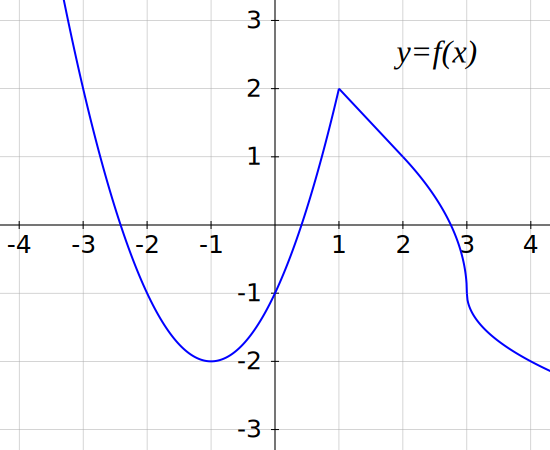
\includegraphics[scale=.4]{G4}
		\end{center}
	\end{frame}
	%-----------------------------

	%QUESTION_INFO: {"unit":3,"question":3,"title":"Derivative from a graph","images":["G4.svg","G4.png"]}
	\begin{frame}[t]
		\frametitle{Derivative from a graph}
		This is the graph of the function $f$. \\ Sketch the graph of its derivative
		$f'$.
		\begin{center}
			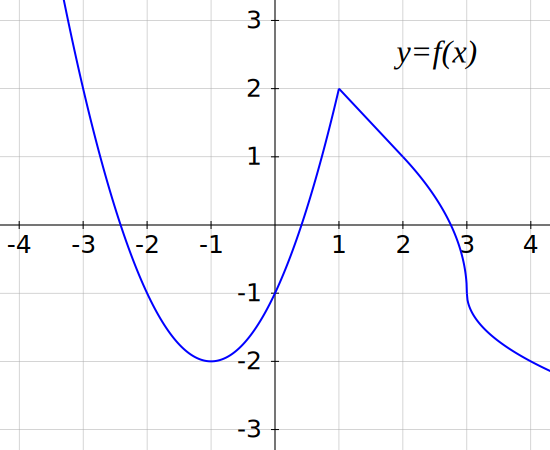
\includegraphics[scale=.4]{G4}
		\end{center}
	\end{frame}

	%-----------------------------

	%QUESTION_INFO: {"unit":3,"question":4,"title":"From the derivative to the function","images":["G5.svg","G5.png"]}
	\begin{frame}[t]
		\frametitle{From the derivative to the function}

		\begin{enumerate}
			\item Sketch the graph of a continuous function with domain $\mathbb{R}$,
				whose derivative has the graph below.

			\item Sketch the graph of a non-continuous function whose derivative has the
				graph below.
		\end{enumerate}

		\begin{center}
			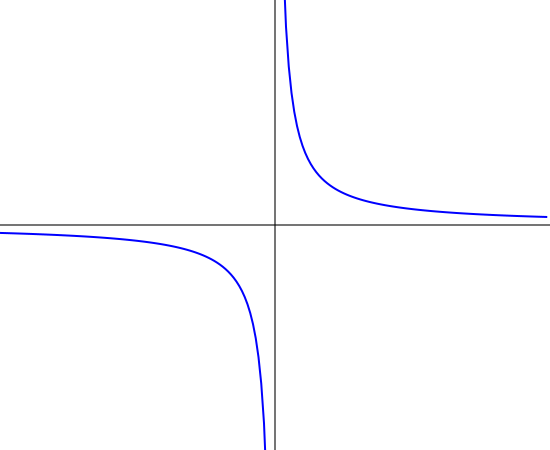
\includegraphics[scale=.3]{G5}
		\end{center}
	\end{frame}

	%-----------------------------

	%QUESTION_INFO: {"unit":3,"question":5,"title":"Estimations - 1","images":[]}
	\begin{frame}
		\frametitle{Estimations - 1}

		Let $f$ be a continuous function with domain $\mathbb{R}$.

		\vfill

		\begin{enumerate}
			\item We know $f(4)=3$ and $f(4.2)=2.2$. \\ Based only on this, give your best
				estimate for $f(4.1)$.
				\vfill

			\item We know $f(4)=3$ and $f'(4)=0.6$. \\ Based only on this, give your best
				estimate for $f(4.1)$.
				\vfill

			\item We know $f(4)=3$ and $f(4.1) = 4$. \\ Based only on this, give your best
				estimate for $f'(4)$.
		\end{enumerate}

		\vfill
	\end{frame}

	%-----------------------------

	%QUESTION_INFO: {"unit":3,"question":6,"title":"Estimations — 2","images":[]}
	\begin{frame}
		\frametitle{Estimations -- 2}

		Without using a calculator, estimate $\displaystyle \sqrt[20]{1.01}$ as well
		as you can.

		\emph{Hint:} You know the value of $\displaystyle f(x) = \sqrt[20]{x}$ and
		its derivative at one point very close to 1.01. Use the tangent line at that
		point as an approximation.
	\end{frame}
	%-----------------------------

	%QUESTION_INFO: {"unit":3,"question":7,"title":"Estimations — 3","images":[]}
	\begin{frame}[t]
		\fontsize{13}{13}\selectfont
		\frametitle{Estimations -- 3}

		%The point of this question is to make them discover L'Hopital's Rule!

		\begin{enumerate}
			\item We know \quad $\displaystyle f(0) = 2, \quad f'(0) = 3, \quad g(0) =
				7, \quad g'(0) = 5.$

				\vspace{.2cm}
				Compute \; $\displaystyle \lim_{x \to 0}\frac{f(x)}{g(x)}$.

				\vfill

			\item We know \quad $\displaystyle f(0) = 0, \quad f'(0) = 3, \quad g(0) =
				0, \quad g'(0) = 5.$

				\vspace{.2cm}
				\begin{itemize}
					\item When $x$ is close to $0$, give estimates for
						$\displaystyle f(x)$ and $\displaystyle g(x)$ using the tangent
						lines at $0$.

					\item Use those estimates to compute \; $\displaystyle \lim_{x \to 0}\frac{f(x)}{g(x)}$.
				\end{itemize}
		\end{enumerate}

		\vfill
	\end{frame}

	%-----------------------------

	%  Derivative from the definition

	%-----------------------------

	%-----------------------------

	%QUESTION_INFO: {"unit":3,"question":8,"title":"Derivatives from the definition","images":[]}
	\begin{frame}[t]
		\frametitle{Derivatives from the definition}

		Let
		\[
			g(x) = \frac{2}{\sqrt{x}}
		\]

		Calculate $\displaystyle g'(4)$ directly from the definition of derivative as
		a limit.
	\end{frame}

	%-----------------------------

	% Derivative as rate of change

	%-----------------------------

	%-----------------------------

	%QUESTION_INFO: {"unit":3,"question":9,"title":"Bella","images":["G9.png"]}
	\begin{frame}
		\frametitle{Bella}

		The graph below describes Bella's distance from home one morning as she
		drives drive between her home and school.\\

		Describe a possible scenario for her travels that morning. \\ Then sketch
		the corresponding graph of his velocity.

		\begin{center}
			\includegraphics[width=0.7\textwidth]{G9}
		\end{center}
	\end{frame}

	%-----------------------------

	%QUESTION_INFO: {"unit":3,"question":10,"title":"Edward and Jacob","images":[]}
	\begin{frame}
		\frametitle{Edward and Jacob}

		Jacob walked at 5 km/h for 20 minutes and then sprinted at 15 km/h for 8
		minutes.
		\begin{enumerate}
			\item How fast would Edward have to walk or run to go the same distance as
				Jacob did in the same time while moving at a constant speed?

			\item Sketch a graph of Jacob's and Edward's positions over time on the same
				set of axes.
		\end{enumerate}
	\end{frame}

	%-----------------------------

	%  Computations

	%-----------------------------

	%-----------------------------

	%QUESTION_INFO: {"unit":3,"question":11,"title":"Computations: Basic differentiation rules","images":[]}
	\begin{frame}
		\frametitle{Computations: Basic differentiation rules}

		Compute the derivative of the following functions:

		\begin{multicols}{2}
			\begin{enumerate}
				\item $\displaystyle f(x) = x^{100}- 3x^{9}- 2$

				\item $\displaystyle f(x) = \sqrt[3]{x}+ 6$

				\item $\displaystyle f(x) = \frac{4}{x^{4}}$

				\item $\displaystyle f(x) = \sqrt{x}\left( 1 + 2x \right)$

				\item $\displaystyle f(x) = \frac{x^{6}+ 1}{x^{3}}$

				\item $\displaystyle f(x) = \frac{x^{2}-2}{x^{2}+2}$
			\end{enumerate}
		\end{multicols}
	\end{frame}

	%-----------------------------

	%QUESTION_INFO: {"unit":3,"question":12,"title":"Computations: Chain rule","images":[]}
	\begin{frame}[t]
		\frametitle{Computations: Chain rule}

		Compute the derivative of

		\begin{enumerate}
			\item $\displaystyle f(x) = \left( 2x^{2}+x+1 \right)^{8}$

			\item $\displaystyle f(x) = \frac{1}{\left( x + \sqrt{x^2+x}\right)^{137}}$
		\end{enumerate}
	\end{frame}
	%-----------------------------

	%QUESTION_INFO: {"unit":3,"question":13,"title":"A long chain","images":[]}
	\begin{frame}[t]
		\frametitle{A long chain}

		The function below has 137 square roots:
		\[
			f(x) = \sqrt{x+ \sqrt{x +
			\sqrt{x + \sqrt{x+ \ldots + \sqrt{x + \sqrt{x+1}}}}}}
		\]

		Find the equation of the line tangent to the graph of $f$ at the point with
		$x$-coordinate $0$.
	\end{frame}

	%-----------------------------

	%QUESTION_INFO: {"unit":3,"question":14,"title":"Computations: Trig derivatives","images":[]}
	\begin{frame}[t]
		\frametitle{Computations: Trig derivatives}

		Compute the derivatives of the following functions:

		\begin{enumerate}
			%	\item  \DS{f(x) = x \sin x}

			\item $\displaystyle f(x) = \tan (3x^{2}+1)$

				\vfill

			\item $\displaystyle f(x) = (\cos x )( \sin 2x )(\tan 3x)$

				\vfill

			\item $\displaystyle f(x) = \cos ( \sin( \tan x))$
				\vfill

			\item $\displaystyle f(x) = \cos \left( 3x + \sqrt{1 + \sin^{2}x^{2}}\right
				)$
				\vfill
			%	\item  \DS{f(x) = \frac{x + \sin x}{x + \cos x}}
		\end{enumerate}
	\end{frame}

	%-----------------------------

	%  Differentiation rules

	%-----------------------------

	%-----------------------------

	%QUESTION_INFO: {"unit":3,"question":15,"title":"Differentiable functions","images":[]}
	\begin{frame}[t]
		\frametitle{Differentiable functions}

		Let $a \in \mathbb{R}$. \\ Let $f$ be a function with domain $\mathbb{R}$.
		\\ Assume $f$ is differentiable everywhere. \\ What can we conclude?

		\begin{multicols}{2}
			\begin{enumerate}
				\item $f(a)$ is defined.

				\item $\displaystyle \lim_{x \to a}f(x)$ exists.

				\item $f$ is continuous at $a$.

				\item $f'(a)$ exists.

				\item $\displaystyle \lim_{x \to a}f'(x)$ exists.

				\item $\displaystyle f'$ is continuous at $a$.
			\end{enumerate}
		\end{multicols}
	\end{frame}

	%-----------------------------

	%QUESTION_INFO: {"unit":3,"question":16,"title":"True or False - Differentiability vs Continuity","images":[]}
	\begin{frame}[t]
		\fontsize{13}{13}\selectfont
		\frametitle{True or False - Differentiability vs Continuity}

		Let $f$ be a function with domain $\mathbb{R}$. Let $c \in \mathbb{R}$. \\ Which
		of these implications are true?

		\vfill

		\begin{enumerate}
			\item IF $f$ is {\color{red} continuous} at $c$, THEN $f$ is
				{\color{blue} differentiable} at $c$
				\vfill

			\item IF $f$ is {\color{blue} differentiable} at $c$, THEN $f$ is
				{\color{red} continuous} at $c$
				\vfill

			\item IF $f$ is {\color{blue} differentiable} at $c$, THEN $f'$ is
				{\color{red} continuous} at $c$
				\vfill

			\item IF $f'$ is {\color{red} continuous} at $c$, THEN $f$ is
				{\color{red} continuous} at $c$
				\vfill

			\item IF $f$ is {\color{blue} differentiable} at $c$, THEN $f$ is
				{\color{red} continuous} at and near $c$.
				\vfill

			\item IF $f$ is {\color{red} continuous} at and near $c$, THEN $f$ is
				{\color{blue} differentiable} at $c$.
				\vfill
		\end{enumerate}
	\end{frame}
	%-----------------------------

	%QUESTION_INFO: {"unit":3,"question":17,"title":"True or False - Differentiability and Operations","images":[]}
	\begin{frame}[t]
		\fontsize{13}{13}\selectfont
		\frametitle{True or False - Differentiability and Operations}

		Let $f$ be a function with domain $\mathbb{R}$. Let $c \in \mathbb{R}$. \\ Let
		$\displaystyle g(x) = f(x)^{2}$. Which of these implications are true?

		\vfill

		\begin{enumerate}
			\item IF $f$ is {\color{blue} differentiable} at $c$, THEN $f+f'$ is
				{\color{red} continuous} at $c$
				\vfill

			\item IF $f$ is {\color{blue} differentiable} at $c$, THEN $3f$ is
				{\color{blue} differentiable} at $c$.
				\vfill

			\item IF $f$ is {\color{blue} differentiable} at $c$, THEN $g$ is
				{\color{blue} differentiable} at $c$.
				\vfill

			\item IF $g$ is {\color{blue} differentiable} at $c$, THEN $f$ is
				{\color{blue} differentiable} at $c$.
				\vfill

			\item IF $f$ is {\color{blue} differentiable} at $c$, THEN $1/f$ is
				{\color{blue} differentiable} at $c$.
				\vfill
		\end{enumerate}
	\end{frame}

	%-----------------------------

	%QUESTION_INFO: {"unit":3,"question":18,"title":"Vertical things","images":[]}
	\begin{frame}[t]
		\frametitle{Vertical things}

		\begin{itemize}
			\item Construct a function $f$ that has a {\color{red} vertical asymptote}
				at $x=2$.

			\item Construct a function $g$ that has a {\color{blue} vertical tangent line}
				at $x=2$.
		\end{itemize}
	\end{frame}

	%-----------------------------

	%QUESTION_INFO: {"unit":3,"question":19,"title":"Absolute value and tangent lines","images":["G8.svg","G8.png"]}
	\begin{frame}[t]
		\frametitle{Absolute value and tangent lines}

		At (0,0) the graph of $\displaystyle y=|x|$...
		\begin{enumerate}
			\item ... has one tangent line: $y=0$

			\item ... has one tangent line: $x=0$

			\item ... has two tangent lines $y=x$ and $y=-x$

			\item ... has no tangent line
		\end{enumerate}

		\begin{center}
			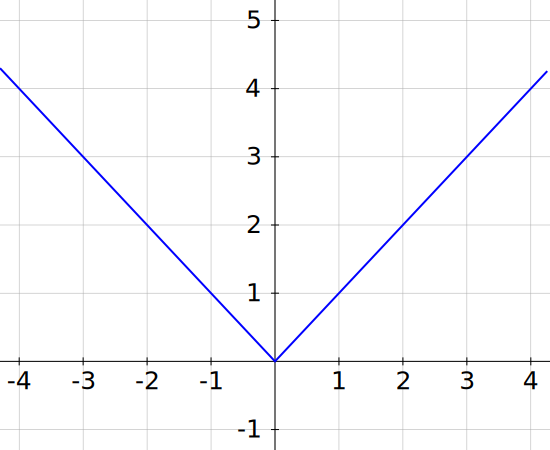
\includegraphics[scale=.25]{G8}
		\end{center}
	\end{frame}

	%-----------------------------

	%QUESTION_INFO: {"unit":3,"question":20,"title":"Absolute value and derivatives - 1","images":[]}
	\begin{frame}[t]
		\frametitle{Absolute value and derivatives - 1}

		Let $h(x) = x|x|$. What is $h'(0)$?

		\begin{enumerate}
			\item It is 0.

			\item It doesn't exist because $|x|$ is not differentiable at $0$.

			\item It doesn't exist because the right- and left-limits, when computing the
				derivative, are different.

			\item It doesn't exist because it has a corner.

			\item It doesn't exist for a different reason.
		\end{enumerate}
	\end{frame}

	%-----------------------------

	%QUESTION_INFO: {"unit":3,"question":21,"title":"Absolute value and derivatives - 2","images":[]}
	\begin{frame}[t]
		\frametitle{Absolute value and derivatives - 2}

		\begin{block}{True or False?}
			For all $n \in \mathbb{Z}$ and all $x$, $\frac{d}{dx}|x|^{n}=nx|x|^{n-2}$.
		\end{block}
	\end{frame}

	%-----------------------------

	%QUESTION_INFO: {"unit":3,"question":22,"title":"Write a proof for the quotient rule for derivatives","images":[]}
	\begin{frame}[t]
		\fontsize{13}{13}\selectfont
		\frametitle{Write a proof for the quotient rule for derivatives}

		\begin{block}{Theorem}
			\begin{itemize}
				\item Let $a \in \mathbb{R}$.

				\item Let $f$ and $g$ be functions defined at and near $a$. \\ Assume
					$g(x) \neq 0$ for $x$ close to $a$.

				\item We define the function $h$ by $\displaystyle h(x) = \frac{f(x)}{g(x)}$.
			\end{itemize}

			IF $f$ and $g$ are differentiable at $a$, \\ THEN $h$ is differentiable at
			$a$, and
			\[
				h'(a) = \frac{f'(a) g(a) - f(a) g'(a)}{g(a)^{2}}.
			\]
		\end{block}

		\vfill

		Write a proof directly from the definition of derivative.

		\emph{Hint:} Imitate the proof of the product rule in Video 3.6.
	\end{frame}

	%-----------------------------

	%QUESTION_INFO: {"unit":3,"question":23,"title":"Check your proof","images":[]}
	\begin{frame}[t]
		\frametitle{Check your proof}

		\begin{enumerate}
			\item Did you use the \emph{definition} of derivative?

			\item Are there words or only equations?

			\item Does every step follow logically?

			\item Did you only assume things you could assume?

			\item Did you assume at some point that a function was differentiable? If
				so, did you justify it?

			\item \label{qu:cont} Did you assume at some point that a function was continuous?
				If so, did you justify it?
		\end{enumerate}

		If you answered ``no" to Q\ref{qu:cont}, you probably missed something
		important.
	\end{frame}
	%-----------------------------

	%QUESTION_INFO: {"unit":3,"question":24,"title":"Critique this proof","images":[]}
	\begin{frame}[t]
		\fontsize{13}{13}\selectfont
		\frametitle{Critique this proof}
		\vspace{-1cm}
		\begin{align*}
			h'(a) \; & = \; \lim_{x \to a}\frac{h(x) - h(a) }{x - a}\; = \; \lim_{x \to a}\frac{\; \dfrac{f(x)}{g(x)} \; - \; \dfrac{f(a)}{g(a)} \;}{x-a} \\
			\         \\
			         & = \; \lim_{x \to a}\frac{f(x)g(a) - f(a)g(x)}{g(x)g(a) \; (x-a)}                                                                   \\
			\         \\
			         & = \; \lim_{x \to a}\frac{f(x)g(a) - f(a)g(a) + f(a)g(a) - f(a) g(x)}{g(x) g(a) \; (x-a)}                                           \\
			\         \\
			         & = \; \lim_{x \to a}\left\{ \left[ \frac{f(x) - f(a)}{x-a}g(a) - f(a) \frac{g(x) - g(a)}{x-a}\right] \frac{1}{g(x) g(a)}\right\}    \\
			\         \\
			         & = \; \left[ f'(a) g(a) - f(a) g'(a) \right] \frac{1}{g(a) g(a)}
		\end{align*}
	\end{frame}

	%-----------------------------

	%  HIGHER ORDER DERIVATIVES

	%-----------------------------

	%-----------------------------

	%QUESTION_INFO: {"unit":3,"question":25,"title":"Higher order derivatives","images":[]}
	\begin{frame}[t]
		\frametitle{Higher order derivatives}

		Let $\displaystyle g(x) = \frac{1}{x^{3}}$.

		\begin{itemize}
			\item Calculate the first few derivatives.

			\item Make a conjecture for a formula for the $n$-th derivative $\displaystyle
				g^{(n)}(x)$.

			\item Prove it by induction.
		\end{itemize}
	\end{frame}

	%-----------------------------

	%QUESTION_INFO: {"unit":3,"question":26,"title":"Nixon","images":[]}
	\begin{frame}
		\frametitle{Nixon}

		Richard Nixon, during the 1972 US Presidential campaign, (paraphrased):

		\begin{quote}
			\emph{Inflation is increasing, but the rate of increase of inflation is decreasing.}
		\end{quote}

		\vfill

		Let
		\begin{itemize}
			\item $C$ = cost of life

			\item $t$ = time
		\end{itemize}
		What did Nixon say in terms of derivatives?

		\vfill
	\end{frame}
	%-----------------------------

	%  CHAIN RULE

	%-----------------------------

	%------------------------------

	%QUESTION_INFO: {"unit":3,"question":27,"title":"Quick composition","images":[]}
	\begin{frame}
		\frametitle{Quick composition}

		Let $f$ and $g$ be differentiable functions and let $h=f\circ g$. \\ What is
		$h^{\prime}(2)$? \begin {enumerate} \item $f^{\prime}(2)\circ g^{\prime}(2)$
		\item $f^{\prime}(2)g^{\prime}(2)$ \item $f^{\prime}(g(2)) g^{\prime}(2)$
		\item $f^{\prime}(g(x)) g^{\prime}(2)$ \end{enumerate}

		%Answer: (c). Even though students may have memorized the Chain Rule formula, some may not be able to apply it to this type of problem.
	\end{frame}

	%-----------------------------

	%QUESTION_INFO: {"unit":3,"question":28,"title":"True or False - Differentiability and Composition","images":[]}
	\begin{frame}[t]
		\frametitle{True or False - Differentiability and Composition}

		Let $f$ and $g$ be functions with domain $\mathbb{R}$. Let $c \in \mathbb{R}$.
		\\ Assume $f$ and $g$ are differentiable at $c$. \\ What can we conclude?

		\vfill

		\begin{enumerate}
			\item $f \circ g$ \; is {\color{blue} differentiable} at $c$.
				\vfill

			\item $f \circ f$ \; is {\color{blue} differentiable} at $c$.
				\vfill

			\item $f \circ \sin$ \; is {\color{blue} differentiable} at $c$.
				\vfill

			\item $\sin \circ f$ \; is {\color{blue} differentiable} at $c$.
				\vfill
		\end{enumerate}
	\end{frame}
	%-----------------------------

	%QUESTION_INFO: {"unit":3,"question":29,"title":"Chain rule from a graph","images":["G10.png"]}
	\begin{frame}
		\frametitle{Chain rule from a graph}

		If $f$ and $g$ are the functions whose graphs are shown. \\ Let $u(x)=f(g(x))$
		and $v(x)=g(f(x))$. \\
		\medskip

		Find each derivative, if it exists. \\ If it does not exist, explain why.

		\begin{enumerate}
			\item $u'(1)$

			\item $v'(1)$
		\end{enumerate}
		\vspace{-1cm}

		\begin{center}
			\includegraphics[width=0.5\textwidth]{G10}
		\end{center}
	\end{frame}

	%-----------------------------

	%QUESTION_INFO: {"unit":3,"question":30,"title":"Balloon","images":["G7.svg","G7.png","G6.svg","G6.png"]}
	\begin{frame}[t]
		\frametitle{Balloon}

		I am inflating a spherical balloon. Below is the graph of the radius $r$ (in
		$cm$) as a function of time $t$ (in $s$). At what rate is the volume of the
		balloon increasing at time $4s$?

		\begin{center}
			\only<1>{
			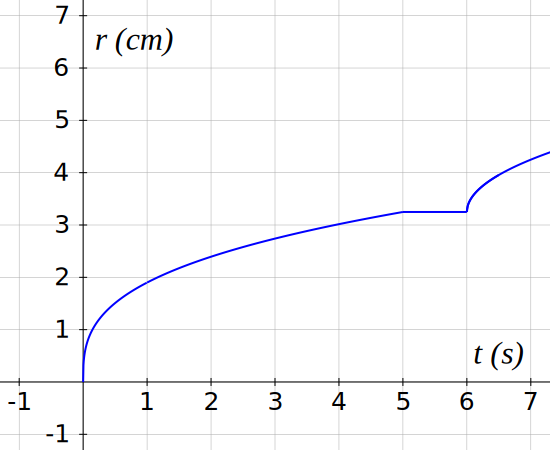
\includegraphics[scale=.35]{G6}
			} \only<2>{
			\includegraphics[scale=.35]{G7}
			}
		\end{center}
	\end{frame}
	%-----------------------------

	%QUESTION_INFO: {"unit":3,"question":31,"title":"An alternative proof of the quotient rule","images":[]}
	\begin{frame}[t]
		\frametitle{An alternative proof of the quotient rule}

		Assume we have already proven the product rule, the power rule, and the
		chain rule.

		Obtain a formula for the derivative of
		$\displaystyle h(x) = \frac{f(x)}{g(x)}$.

		\emph{Hint:} $\displaystyle \frac{f(x)}{g(x)}= f(x) \cdot g(x)^{-1}$
	\end{frame}

	%-----------------------------

	%QUESTION_INFO: {"unit":3,"question":32,"title":"Derivatives of $\\displaystyle (f \\circ g)$","images":[]}
	\begin{frame}
		\frametitle{Derivatives of $\displaystyle (f \circ g)$}

		Assume $f$ and $g$ are functions that have all their derivatives. Find formulas
		for
		\begin{enumerate}
			\item $\displaystyle (f \circ g)'(x)$

			\item $\displaystyle (f \circ g)''(x)$

			\item $\displaystyle (f \circ g)'''(x)$
		\end{enumerate}

		in terms of the values of $f$, $g$ and their derivatives.

		\emph{Hint:} The first one is simply the chain rule.

		\
		% \pause

		\emph{Challenge:} Find a formula for $\displaystyle (f \circ g)^{(n)}(x)$ \\
		(This is beyond the scope of this course).
	\end{frame}

	%-----------------------------

	%  TRIG

	%-----------------------------

	%-----------------------------

	%QUESTION_INFO: {"unit":3,"question":33,"title":"Derivative of $\\cos$","images":[]}
	\begin{frame}[t]
		\frametitle{Derivative of $\cos$}

		Let $\displaystyle g(x) = \cos x.$

		Obtain and prove a formula for its derivative directly from the definition of
		derivative as a limit.

		\vfill

		{\bfseries Hint:} Imitate the derivation in Video 3.12. \\ If you need a trig
		identity that you do not know, google it or ask another student.

		%{\bf Hint:}  This identity may come in handy:

		%	$$

		%		\cos (a + b) = \cos a \cos b - \sin a \sin b

		%	$$
	\end{frame}

	%-----------------------------

	%QUESTION_INFO: {"unit":3,"question":34,"title":"Derivatives of the other trig functions","images":[]}
	\begin{frame}[t]
		\frametitle{Derivatives of the other trig functions}

		Use the basic differentiation rules, as well as
		\[
			\frac{d}{dx}\sin x = \cos x, \quad \quad \frac{d}{dx}\cos x = - \sin x,
		\]
		to quickly obtain and prove formulas for the derivatives of $\tan$, $\cot$, $\sec$,
		and $\csc$.
	\end{frame}

	%-----------------------------

	%QUESTION_INFO: {"unit":3,"question":35,"title":"Product of trig functions","images":[]}
	\begin{frame}
		\frametitle{Product of trig functions}

		Let $f(x)= \sin x \cos x$. What is its derivative $f'(x)$?
		\begin{enumerate}
			\item $1-2\sin^{2}(x)$

			\item $2\cos^{2}(x) -1$

			\item $\cos 2x$

			\item all of the above

			\item none of the above
		\end{enumerate}

		%Answer: (d).} (a) - (c) are equivalent formulae. One can get (a) by using the product rule and $\cos^2(x)=1-\sin ^2(x)$.
	\end{frame}

	%-----------------------------

	%QUESTION_INFO: {"unit":3,"question":36,"title":"A pesky function","images":[]}
	\begin{frame}[t]
		\frametitle{A pesky function}

		Let $\displaystyle h(x) =
		\begin{cases}
			x^{2}\sin \dfrac{\;1\;}{x} & \text{ if }x \neq 0 \\
			0                          & \text{ if }x=0
		\end{cases}$.

		\begin{enumerate}
			\item Calculate $\displaystyle h'(x)$ for any $x \neq 0$.

			\item \label{it:0a} Using the definition of derivative, calculate
				$\displaystyle h'(0)$.

			\item \label{it:0b} Calculate $\displaystyle \lim_{x \to 0}h'(x)$

				\vspace{.2cm}
				{\fontsize{13}{13}\selectfont \emph{Hint:} Questions \ref{it:0a} and \ref{it:0b} have different answers.}

				% \pause
				\vspace{.2cm}

			\item Is $h$ continuous at $0$?

			\item Is $h$ differentiable at $0$?

			\item Is $h'$ continuous at $0$?
		\end{enumerate}
	\end{frame}
	%-----------------------------

	%  IMPLICIT DIFFERENTIATION

	%-----------------------------

	%-----------------------------

	%QUESTION_INFO: {"unit":3,"question":37,"title":"Implicit differentiation","images":[]}
	\begin{frame}[t]
		\frametitle{Implicit differentiation}

		The equation
		\[
			\sin (x+y) + xy^{2}= 0
		\]
		defines a function $\displaystyle y=h(x)$ near $(0,0)$. \href{https://www.desmos.com/calculator/bvupq00r6s}{\beamergotobutton{graph}}

		Using implicit differentiation, compute
		\begin{multicols}{4}
			\begin{enumerate}
				\item $\displaystyle h(0)$

				\item $\displaystyle h'(0)$

				\item $\displaystyle h''(0)$

				\item $\displaystyle h'''(0)$
			\end{enumerate}
		\end{multicols}
	\end{frame}

	%------------------------------

	%-----------------------------
\end{document}
%-----------------------------

%-----------------------------